\XtoCBlock{MinMaxPeriodic}
\label{block:MinMaxPeriodic}
\begin{figure}[H]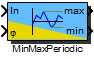
\includegraphics{MinMaxPeriodic}\end{figure} 

\begin{XtoCtabular}{Inports}
In & Input signal\tabularnewline
\hline
phi & Angle signal\tabularnewline
\hline
\end{XtoCtabular}


\begin{XtoCtabular}{Outports}
max & Maximum of input signal\tabularnewline
\hline
min & Minimum of input signal\tabularnewline
\hline
\end{XtoCtabular}

\subsubsection*{Description:}
Outputs the minimum and maximum of the input signal over one period of the (angle) signal phi.

% include optional documentation file
\InputIfFileExists{\XcHomePath/Library/General/Doc/MinMaxPeriodic_Info.tex}{\vspace{1ex}}{}

\subsubsection*{Implementations:}
\begin{tabular}{l l}
\textbf{FiP8} & 8 Bit Fixed Point Implementation\tabularnewline
\textbf{FiP16} & 16 Bit Fixed Point Implementation\tabularnewline
\textbf{FiP32} & 32 Bit Fixed Point Implementation\tabularnewline
\textbf{Float32} & 32 Bit Floating Point Implementation\tabularnewline
\textbf{Float64} & 64 Bit Floating Point Implementation\tabularnewline
\end{tabular}

\XtoCImplementation{FiP8}
\index{Block ID!464}
\nopagebreak[0]
% Implementation details
\begin{tabular}{l l}
\textbf{Name} & FiP8 \tabularnewline
\textbf{ID} & 464 \tabularnewline
\textbf{Revision} & 0.1 \tabularnewline
\textbf{C filename} & MinMaxPeriodic\_FiP8.c \tabularnewline
\textbf{H filename} & MinMaxPeriodic\_FiP8.h \tabularnewline
\end{tabular}
\vspace{1ex}

8 Bit Fixed Point Implementation

\begin{XtoCtabular}{Controller Parameters}
min\_act & Current minimum\tabularnewline
\hline
max\_act & Current maximum\tabularnewline
\hline
phi\_old & Angle signal from previous cycle\tabularnewline
\hline
\end{XtoCtabular}

% Implementation data structure
\XtoCDataStruct{Data Structure:}
\begin{lstlisting}
typedef struct {
     uint16        ID;
     int8          *In;
     int8          *phi;
     int8          max;
     int8          min;
     int8          min_act;
     int8          max_act;
     int8          phi_old;
} MINMAXPERIODIC_FIP8;
\end{lstlisting}

\ifdefined \AddTestReports
\InputIfFileExists{\XcHomePath/Library/General/Doc/Test_MinMaxPeriodic_FiP8.tex}{}{}
\fi
\XtoCImplementation{FiP16}
\index{Block ID!465}
\nopagebreak[0]
% Implementation details
\begin{tabular}{l l}
\textbf{Name} & FiP16 \tabularnewline
\textbf{ID} & 465 \tabularnewline
\textbf{Revision} & 0.1 \tabularnewline
\textbf{C filename} & MinMaxPeriodic\_FiP16.c \tabularnewline
\textbf{H filename} & MinMaxPeriodic\_FiP16.h \tabularnewline
\end{tabular}
\vspace{1ex}

16 Bit Fixed Point Implementation

\begin{XtoCtabular}{Controller Parameters}
min\_act & Current minimum\tabularnewline
\hline
max\_act & Current maximum\tabularnewline
\hline
phi\_old & Angle signal from previous cycle\tabularnewline
\hline
\end{XtoCtabular}

% Implementation data structure
\XtoCDataStruct{Data Structure:}
\begin{lstlisting}
typedef struct {
     uint16        ID;
     int16         *In;
     int16         *phi;
     int16         max;
     int16         min;
     int16         min_act;
     int16         max_act;
     int16         phi_old;
} MINMAXPERIODIC_FIP16;
\end{lstlisting}

\ifdefined \AddTestReports
\InputIfFileExists{\XcHomePath/Library/General/Doc/Test_MinMaxPeriodic_FiP16.tex}{}{}
\fi
\XtoCImplementation{FiP32}
\index{Block ID!466}
\nopagebreak[0]
% Implementation details
\begin{tabular}{l l}
\textbf{Name} & FiP32 \tabularnewline
\textbf{ID} & 466 \tabularnewline
\textbf{Revision} & 0.1 \tabularnewline
\textbf{C filename} & MinMaxPeriodic\_FiP32.c \tabularnewline
\textbf{H filename} & MinMaxPeriodic\_FiP32.h \tabularnewline
\end{tabular}
\vspace{1ex}

32 Bit Fixed Point Implementation

\begin{XtoCtabular}{Controller Parameters}
min\_act & Current minimum\tabularnewline
\hline
max\_act & Current maximum\tabularnewline
\hline
phi\_old & Angle signal from previous cycle\tabularnewline
\hline
\end{XtoCtabular}

% Implementation data structure
\XtoCDataStruct{Data Structure:}
\begin{lstlisting}
typedef struct {
     uint16        ID;
     int32         *In;
     int32         *phi;
     int32         max;
     int32         min;
     int32         min_act;
     int32         max_act;
     int32         phi_old;
} MINMAXPERIODIC_FIP32;
\end{lstlisting}

\ifdefined \AddTestReports
\InputIfFileExists{\XcHomePath/Library/General/Doc/Test_MinMaxPeriodic_FiP32.tex}{}{}
\fi
\XtoCImplementation{Float32}
\index{Block ID!467}
\nopagebreak[0]
% Implementation details
\begin{tabular}{l l}
\textbf{Name} & Float32 \tabularnewline
\textbf{ID} & 467 \tabularnewline
\textbf{Revision} & 0.1 \tabularnewline
\textbf{C filename} & MinMaxPeriodic\_Float32.c \tabularnewline
\textbf{H filename} & MinMaxPeriodic\_Float32.h \tabularnewline
\end{tabular}
\vspace{1ex}

32 Bit Floating Point Implementation

\begin{XtoCtabular}{Controller Parameters}
min\_act & Current minimum\tabularnewline
\hline
max\_act & Current maximum\tabularnewline
\hline
phi\_old & Angle signal from previous cycle\tabularnewline
\hline
\end{XtoCtabular}

% Implementation data structure
\XtoCDataStruct{Data Structure:}
\begin{lstlisting}
typedef struct {
     uint16        ID;
     float32       *In;
     float32       *phi;
     float32       max;
     float32       min;
     float32       min_act;
     float32       max_act;
     float32       phi_old;
} MINMAXPERIODIC_FLOAT32;
\end{lstlisting}

\ifdefined \AddTestReports
\InputIfFileExists{\XcHomePath/Library/General/Doc/Test_MinMaxPeriodic_Float32.tex}{}{}
\fi
\XtoCImplementation{Float64}
\index{Block ID!468}
\nopagebreak[0]
% Implementation details
\begin{tabular}{l l}
\textbf{Name} & Float64 \tabularnewline
\textbf{ID} & 468 \tabularnewline
\textbf{Revision} & 0.1 \tabularnewline
\textbf{C filename} & MinMaxPeriodic\_Float64.c \tabularnewline
\textbf{H filename} & MinMaxPeriodic\_Float64.h \tabularnewline
\end{tabular}
\vspace{1ex}

64 Bit Floating Point Implementation

\begin{XtoCtabular}{Controller Parameters}
min\_act & Current minimum\tabularnewline
\hline
max\_act & Current maximum\tabularnewline
\hline
phi\_old & Angle signal from previous cycle\tabularnewline
\hline
\end{XtoCtabular}

% Implementation data structure
\XtoCDataStruct{Data Structure:}
\begin{lstlisting}
typedef struct {
     uint16        ID;
     float64       *In;
     float64       *phi;
     float64       max;
     float64       min;
     float64       min_act;
     float64       max_act;
     float64       phi_old;
} MINMAXPERIODIC_FLOAT64;
\end{lstlisting}

\ifdefined \AddTestReports
\InputIfFileExists{\XcHomePath/Library/General/Doc/Test_MinMaxPeriodic_Float64.tex}{}{}
\fi
